%%%%%%%%%%%%%%%%%%%%%%%%%%%%%%%%%%%%%%%%%%%%%%%%%%%%%
%%% Task 2 %%%%%%%%%%%%%%%%%%%%%%%%%%%%%%%%%%%%%%%%%%
%%%%%%%%%%%%%%%%%%%%%%%%%%%%%%%%%%%%%%%%%%%%%%%%%%%%%
\task{Permanent magnet DC machine} %Oliver

%%%%%%%%%%%%%%%%%%%%%%%%%%%%%%%%%%%%%%%%%%%%%%
\taskGerman{Permanentmagnet-Gleichstrommaschine}
%%%%%%%%%%%%%%%%%%%%%%%%%%%%%%%%%%%%%%%%%%%%%%%

Permanent magnet DC (PMDC) machines are often used in low power applications, such as machine tools or micromobility. In those applications, low voltage ratings are common to ensure safety, in particular regarding touch protection. In the following, you will analyze the operation behavior of a PMDC machine with the parameters given in \autoref{tab:characteristicsPMDC_task2} for an electric scooter application. A gearbox for torque and speed adaptation can be neglected.

\begin{germanblock}
    Die Permanentmagnet-Gleichstrommaschine (PMDC) wird häufig in Niedrigleistungsanwendungen wie Werkzeugmaschinen oder Mikromobilität eingesetzt. In diesen Anwendungen sind Kleinschutzspannungen üblich, um die Sicherheit, insbesondere den Berührungsschutz, zu gewährleisten. Im Folgenden analysieren Sie das Betriebsverhalten einer PMDC-Maschine mit den in \autoref{tab:characteristicsPMDC_task2} angegebenen Parametern für eine Elektroscooter-Anwendung. Ein Getriebe zur Anpassung der Drehzahl und des Drehmoments kann vernachlässigt werden.
\end{germanblock}
\begin{table}[htb]
    \caption{PMDC machine parameters.}
    \centering
    \begin{tabular}{lll}\toprule
        Symbol              & Description         & Values                     \\
        \midrule
        $U_{\mathrm{n}}$    & Nominal voltage     & $\SI{48}{\volt}$           \\
        $I_{\mathrm{n}}$    & Nominal current     & $\SI{5.75}{\ampere}$       \\
        $T_{\mathrm{n}}$    & Nominal torque      & $\SI{1.67}{\newton\meter}$ \\
        $P_{\mathrm{me,n}}$ & Nominal mech. power & $\SI{200}{\watt}$          \\
        $R_\mathrm{a}$      & Armature resistance & \SI{2.4}{\ohm}             \\
        $L_\mathrm{a}$      & Armature inductance & \SI{3.7}{\henry}           \\
        \bottomrule
    \end{tabular}
    \label{tab:characteristicsPMDC_task2}
\end{table}


\subtask{Draw the equivalent circuit diagram of a PMDC machine.}{1}

\subtaskGerman{Zeichnen Sie das Ersatzschaltbild der PMDC-Maschine.}

\begin{solutionblock}
    Since the PMDC machine does not have a distinct field winding, the equivalent circuit diagram boils down to the armature circuit as shown in \autoref{fig:ECD_PMDC}.
    \begin{solutionfigure}[ht]
        \centering
        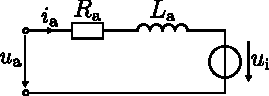
\includegraphics[width=0.45\linewidth]{fig/ECD_PMDC.pdf}
        \caption{Equivalent circuit diagram of the PMDC machine.}
        \label{fig:ECD_PMDC}
    \end{solutionfigure}
\end{solutionblock}

\subtask{Determine the effective PM flux linkage $\psi'_\mathrm{f}$ for the nominal steady-state operating point.}{1}%
\begin{hintblock}
    if and if only you are not able to solve this task, use $\psi'_\mathrm{f} = \SI{0.4}{\volt\second}$ as a substitute result for the subsequent tasks.
\end{hintblock}

\subtaskGerman{Bestimmen Sie die effektive, permanenterregte Flussverkettung $\psi'_\mathrm{f}$ für den nominellen Arbeitspunkt im stationären Zustand.}%
\begin{germanhintblock}
    nur für den Fall, dass Sie kein Ergebnis ermitteln können, verwenden Sie $\psi'_\mathrm{f} =\SI{0.4}{\volt\second}$ für die nachfolgenden Aufgaben.
\end{germanhintblock}


\begin{solutionblock}
    The effective PM flux linkage can be derived from the machine's nominal torque and current:
    $$
        \psi'_\mathrm{f,n} = \frac{T_\mathrm{n}}{I_\mathrm{n}}=\SI{0.29}{\volt\second}.
    $$
\end{solutionblock}

\subtask{What is the machine's nominal speed $n_\mathrm{n}$ and efficiency $\eta_\mathrm{n}$?}{2}
\subtaskGerman{Wie hoch ist die Nenndrehzahl $n_\mathrm{n}$ und der nominelle Wirkungsgrad $\eta_\mathrm{n}$ der Maschine?}


\begin{solutionblock}
    First, the induced voltage is calculated via
    $$
        U_\mathrm{i,n} = U_\mathrm{n} - R_\mathrm{a} I_\mathrm{n} = \SI{34.2}{\volt}.
    $$
    The nominal angular velocity is
    $$
        \omega_\mathrm{n} = \frac{U_\mathrm{i,n}}{\psi'_\mathrm{f,n}} = \SI{117.9}{\per\second}
    $$
    resulting in
    $$
        n_\mathrm{n} = \omega_\mathrm{n} \frac{60}{2\pi}\frac{\si{\second}}{\si{\minute}} = \SI{1126.2}{\per\minute}.
    $$
    For determining the nominal efficiency, we first calculate the nominal electrical power
    $$
        P_\mathrm{el,n} = U_\mathrm{n}I_\mathrm{n} = \SI{276}{\watt}
    $$
    and then use the already known nominal mechanical power to receive
    $$
        \eta_\mathrm{n} = \frac{P_\mathrm{me,n}}{P_\mathrm{el,n}} = \SI{72.46}{\percent}.
    $$
\end{solutionblock}

\subtask{Assume that  the scooter's load torque $T_\mathrm{L}$ is quadratically depending on the speed since the air drag is dominant. This is represented via the equation below utilizing the friction coefficient $b$ with:
    $$
        T_\mathrm{L}(\omega) = b \omega^2 \quad \mbox{with} \quad b = \SI{0.001}{\newton\meter\second^2}.
    $$
    Calculate the resulting operating point assuming the scooter drive is powered with the fixed, nominal voltage.}{3}
\subtaskGerman{Angenommen das Lastmoment $T_\mathrm{L}$ des Scooters hängt quadratisch von der Drehzahl ab, da der Luftwiderstand dominant ist. Dies wird über die folgende Gleichung unter Verwendung des Reibungskoeffizienten $b$ mit
    $$
        T_\mathrm{L}(\omega) = b \omega^2 \quad \mbox{mit} \quad b = \SI{0.001}{\newton\meter\second^2}
    $$

    dargestellt. Berechnen Sie den resultierenden Arbeitspunkt, vorausgesetzt, der Scooterantrieb wird mit der konstanten, nominellen Spannung betrieben.}




\begin{solutionblock}
    The yet unknown operation point is determined by the intersection of the load torque and the machine's torque, which is given by
    $$
        T(\omega) = I_\mathrm{a} \psi'_\mathrm{f} = \frac{U_\mathrm{n} - \omega \psi'_\mathrm{f}}{R_\mathrm{a}} \psi'_\mathrm{f}\stackrel{!}{=} b \omega^2 = T_\mathrm{L}(\omega).
    $$
    Resorting delivers a quadratic equation in $\omega$:
    $$
        b \omega^2 + \frac{{\psi'_\mathrm{f}}^2}{R_\mathrm{a}}\omega - \frac{\psi'_\mathrm{f}U_\mathrm{n}}{R_\mathrm{a}} = 0.
    $$
    The possible solutions of this equation are given by
    $$
        \omega_{1,2} = -\frac{{\psi'_\mathrm{f}}^2}{2bR_\mathrm{a}} \pm \sqrt{\left(\frac{{\psi'_\mathrm{f}}^2}{2bR_\mathrm{a}}\right)^2 + \frac{\psi'_\mathrm{f}U_\mathrm{n}}{bR_\mathrm{a}}}.
    $$
    The positive solution is the relevant one, which results in
    $$
        \omega = \SI{60.63}{\per\second}, \quad n= \SI{578.94}{\per\minute}.
    $$
    The corresponding load torque is given by
    $$
        T_\mathrm{L} = b \omega^2 = \SI{3.68}{\newton\meter}.
    $$
    The machine's armature current is calculated by
    $$
        I_\mathrm{a} = \frac{U_\mathrm{n} - \omega \psi'_\mathrm{f}}{R_\mathrm{a}} = \SI{12.67}{\ampere}.
    $$
\end{solutionblock}


\subtask{What is the theoretical maximum speed of the PMDC machine if unloaded? Discuss why this maximum speed is an inherent limitation of the PMDC machine.}{2}
\subtaskGerman{Wie hoch ist die theoretische Höchstdrehzahl der PMDC-Maschine im Leerlauf? Diskutieren Sie, warum diese Höchstdrehzahl eine inhärente Begrenzung der PMDC-Maschine ist.}
\begin{solutionblock}
    During no-load operation, the armature current is zero, which results in the induced voltage being equal to the nominal voltage:
    $$
        U_\mathrm{i} = U_\mathrm{n} = \omega \psi'_\mathrm{f}.
    $$
    Rearranging this equation delivers the theoretical maximum speed:
    $$
        \omega_\mathrm{max} = \frac{U_\mathrm{n}}{\psi'_\mathrm{f}} = \SI{165.52}{\per\second}, \quad n_\mathrm{max} = \SI{1580.57}{\per\minute}.
    $$
    The maximum speed is an inherent limitation of the PMDC machine since the induced voltage is proportional to the speed and the flux linkage. If the speed exceeds this limit, the induced voltage would exceed the nominal voltage, which is not possible in practice. Also, a field weakening is not possible due to the permanent magnet excitation, i.e., the flux linkage is constant and cannot be reduced to increase the speed.
\end{solutionblock}